\documentclass[12pt,a4paper]{article}
\usepackage[a4paper, total={6.95in, 9.7in}]{geometry}
\usepackage[utf8]{inputenc}
\usepackage{graphicx}
\usepackage{amsmath}
\usepackage{amssymb}
\usepackage{amsthm}
\usepackage{subfigure}
\usepackage{bm}
\usepackage{listings}
\setlength{\parindent}{0pt}


\author{\vspace{1mm}
  Paul Hill}

\date{\vspace{1mm} % Datumsfeld einrichten
       \today}

\thispagestyle{empty} % Die Titelseite soll keine Seitenzahl bekommen...[1]
%\end{titlepage}


\title{Neuro-Backprop}
\date{August 2020}

\begin{document}

\maketitle

\begin{figure*}[!ht]
  \centering
  \subfigure[random caption 1]{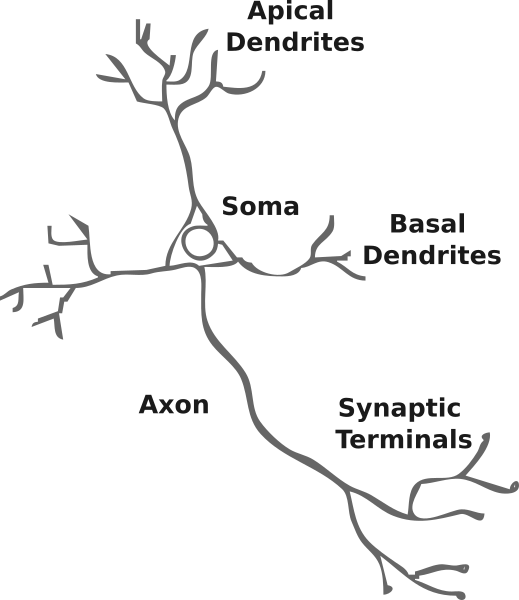
\includegraphics[height=0.35\linewidth]{img/pyramidial.png}}\quad
  \subfigure[random caption 2]{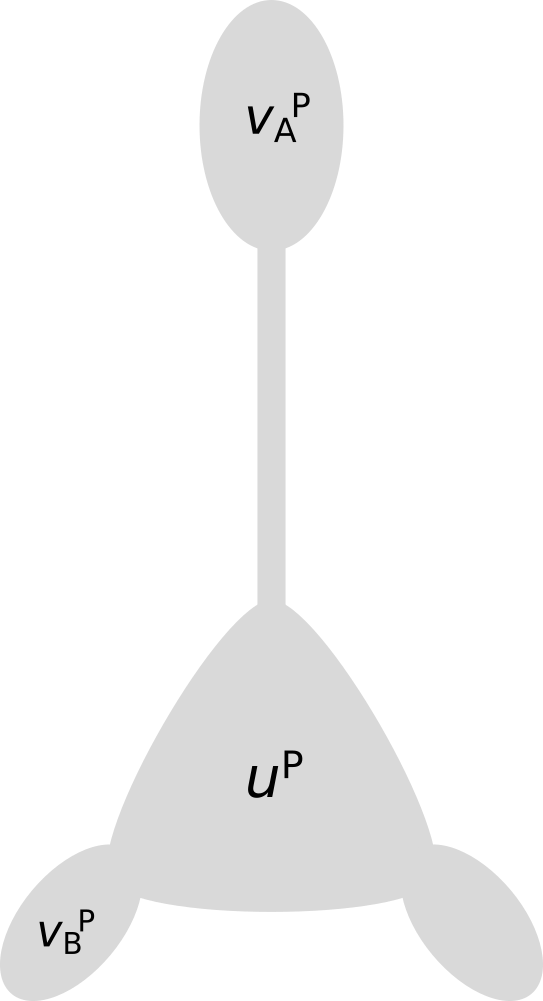
\includegraphics[height=0.35\linewidth]{img/pyr_abstract.png}}\quad
  \subfigure[random caption 1]{
\includegraphics[height=0.35\linewidth]{img/inter.png}}\quad
  \subfigure[random caption 2]{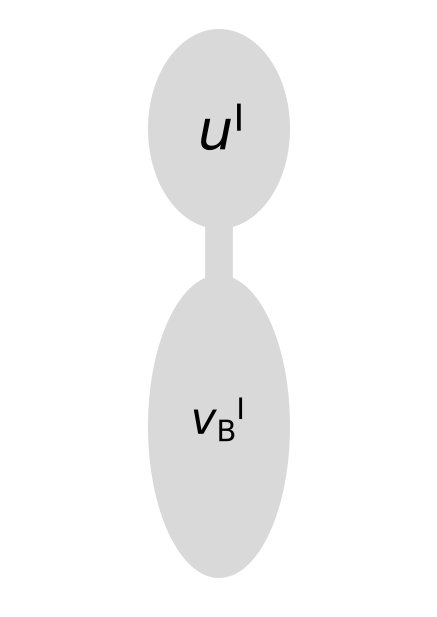
\includegraphics[height=0.2\linewidth]{img/inter_abstract.png}}
\end{figure*}

\section{Introduction}
\subsection{Multicompartment-Neurons}
Real nerve-cells usually have a spatial extension much larger than their actual cell-bodies (somas). To model the spatial variation of electric potentials over such cells (specifically the cell's dendrites), which is due to the finite speed with which electric signals propagate, one introduces several distinct compartments that are coupled to each other. The potential of the soma-compartment is then given by
\begin{equation}
\dot{u} = -g_lu + \sum_xg_x(v_x-u) + I_{syn}, \label{eq:soma}
\end{equation}  
where $g_l$ is the leakage conductance of the soma, $x$ runs over all connected compartments of the cell and $g_x$ is the respective conductance coupling $x$ to the soma. $I_{syn}$ accounts for an additional current input coupled directly into the soma. In our case we will always have $I_{syn} = g_{som}(u_{ex}-u)$, where $u_{ex}$ is any external potential.\\
Note that \eqref{eq:soma} behaves as a low-pass filter for the potentials $u_x$ and $u_{ex}$ with time constant $\tau = \frac{1}{g_{tot}} = \frac{1}{g_l + \sum_x g_x + g_{som}}$. For imprinted signals with time scale $T\gg\tau$ the soma potentials takes on the form (steady-state solution)
\begin{equation}
\tilde{u} = \frac{1}{g_{tot}}\left(\sum_x g_xu_x + g_{som}u_{ex}\right). \label{eq:steady}
\end{equation}

Furthermore we restrict our model to the rate-based case in which synaptic inputs are given in terms of the firing rates of their presynaptic partners $r_y$
\begin{equation}
v_x = \sum_yW_{xy}r_y = \sum_yW_{xy}\phi(u_y).
\end{equation}
Here the vector $\bm{W}_x$ denotes the coupling between the the presynaptic partners and the $x$-compartment and firing rates are given in terms of the corresponding soma potentials $u_y$ via the activation function $\phi(u_y)$.

\subsection{PyraL-Network }
The network approximating the backpropagation-algorithm is built upon two kind of neurons, pyrimidial- and lateral inter-neurons. The first one consists of two compartments beside the soma, the basal and apical dendrites. \eqref{eq:soma} takes on the form
\begin{equation}
\dot{u}^P = -g_lu^P + g_B(v^P_B - u^P) + g_A(v^P_A - u^P), 
\end{equation}
where $B$ denotes the basal and $A$ the apical compartment.
The inter-neurons on the other hand are governed by
\begin{equation}
\dot{u}^I = -g_lu^I + g_D(v^I_D - u^I) + g_{som}(u_{ex} - u^I),
\end{equation}
where $D$ denotes the dendritic compartment and we have an external potential $u_{ex}$ directly coupled into the soma. Fig. ???? depicts both neuron types in their biological manifestation and abstract description, respectively.

With these two types of neurons one is now able to go on and build larger networks as the one depicted in Fig. \ref{fig:network}.

\begin{figure*}[!ht]
  \centering
  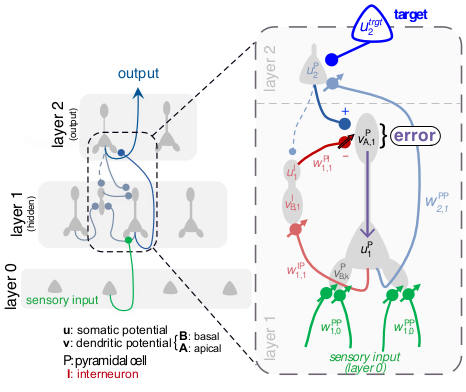
\includegraphics[height=0.6\linewidth]{img/network.png}
  \label{fig:network}
\end{figure*}

The network dynamics for $N$ layers ($N-2$ hidden layers) are governed by the following set of equations (for $0<k<N$) 
\begin{align}
\dot{\bm{u}}^P_k &= -g_l\bm{u}^P_k + g_B(\bm{v}^P_{B,k} - \bm{u}^P_k) + g_A(\bm{v}^P_{A,k} - \bm{u}^P_k)\label{eq:dyn_hidden}\\
\dot{\bm{u}}^I_k &= -g_l\bm{u}^I_k + g_D(\bm{v}^I_{D,k} - \bm{u}^I_k) + g_{som}(\bm{u}^P_{k+1} - \bm{u}^I_k)\\
\bm{v}^P_{B,k} &= \bm{W}^{up}_k\phi(\bm{u}^P_{k-1})\\
\bm{v}^P_{A,k} &= \bm{W}^{pi}_k\phi(\bm{u}^I_{k}) + \bm{W}^{down}_k\phi(\bm{u}^P_{k+1})\label{eq:apical}\\
\bm{v}^I_{D,k} &= \bm{W}^{ip}_k\phi(\bm{u}^P_{k}),
\end{align}
where $\bm{W}$ are now matrices, $\bm{v},\bm{u}$ are vectors and $k$ is the layer index ($k=0$ is the input layer).\\
The output neurons look slightly different,
\begin{align}
\dot{\bm{u}}^P_N &= -g_l\bm{u}^P_N + g_B(\bm{v}^P_{B,N} - \bm{u}^P_N) + g_{som}(\bm{u}^{target} - \bm{u}^P_N)\\
\bm{v}^P_{B,N} &= \bm{W}^{up}_N\phi(\bm{u}^P_{N-1}).\label{eq:dyn_out}
\end{align}

Note that, provided the network reaches a (unique) fix-point, i.e. a configuration in which all derivatives of the soma potentials vanish simultaneously, the network essentially maps the input rates (or input potentials) of the $0$-th layer to the output rates obtained from the $N$-th layer. It is this non-linear mapping between input and output rates that eventually enables the network to solve complex classification and regression tasks by adjusting the strength of its synaptic connections $\bm{W}$. However, the existence (and uniqueness) of a fix-point of the underlaying network dynamics depends non-trivially on the weights $\bm{W}$ and conductances $g$. 

\subsection{Learning-Rules}
Assuming the network indeed converges to a stable fix-point for the given input rates, there is yet no mechanism that makes the output potentials reproduce a given target signal $\bm{u}^{target}$. To solve this the concept of dendritic prediction of somatic spiking rates is introduced. Consider therefore a pyramidial neuron in the output layer when teaching is disabled ($g_{som}=0$). The soma potential is then, in steady-state, given by
\begin{equation}
\hat{\bm{v}}^P_{B,N} \equiv \tilde{\bm{u}}^P = \frac{g_B}{g_l + g_B}\bm{W}r^P_{N-1}.
\end{equation} 
When teaching is enabled, $\tilde{u}^P$ is nudged away from the dendritic prediction $\hat{v}^P$ towards
\begin{equation}
\tilde{\bm{u}}^P_N = (1-\lambda_{out})\hat{\bm{v}}^P_{B,N} + \lambda_{out}\bm{u}^{target},\label{eq:out_stead}
\end{equation}
with $\lambda_{out} = \frac{g_{som}}{g_l + g_B + g_{som}}$.
The difference in predicted and actual firing rate $\phi(u^P) - \phi(\hat{v}^P)$ can now be used to update the synaptic strengths such that $\hat{v}^P$ is itself nudged towards $u^{target}$ and eventually $\tilde{u}^P = \hat{v}^p$ holds again.\\
Similar equations hold for hidden pyramidial neurons and inter-neurons as well
\begin{align}
\tilde{u}^P_k &= \hat{\bm{v}}^P_{B,k} + \lambda_{hid}\bm{v}^P_{A,k}\\ \lambda_{hid} &= \frac{g_A}{g_l + g_B + g_A}\\
\hat{\bm{v}}^P_{B,k} &= \frac{g_B}{g_l + g_B + g_A}\bm{W}^{up}_kr^P_{k-1}\label{eq:basal_pyr}\\
\tilde{u}^I_k &= (1-\lambda_I)\hat{v}^I_{D,k} + \lambda_{I}u^P_{k+1}\\ \lambda_{I} &= \frac{g_{som}}{g_l + g_D + g_{som}}\\
\hat{\bm{v}}^I_{D,k} &= \frac{g_D}{g_l + g_D}\bm{W}^{ip}_kr^P_k \label{eq:dend_int}.
\end{align}

Finally, updating of the weights is realized by first low-pass filtering the dendritic prediction error with time constant $\tau_w$
\begin{align}
\tau_w\dot{\bm{\Delta}}^{up}_k &= \left(\phi(\bm{u}^P_k - \phi(\hat{\bm{v}}^P_{B,k})\right)(r^P_{k-1})^T\label{eq:delta_up}\\
\tau_w\dot{\bm{\Delta}}^{ip}_k &= \left(\phi(\bm{u}^I_k - \phi(\hat{\bm{v}}^I_{D,k})\right)(r^P_{k})^T\\
\tau_w\dot{\bm{\Delta}}^{pi}_k &= -\bm{v}^P_A(r^I_{k})^T \label{eq:delta_ap}
\end{align}
and then integrating
\begin{align}
\frac{d\bm{W}^{up}_k}{dt} &= \eta^{up}_k\bm{\Delta}^{up}_k \\
\frac{d\bm{W}^{ip}_k}{dt} &= \eta^{ip}_k\bm{\Delta}^{ip}_k \\
\frac{d\bm{W}^{pi}_k}{dt} &= \eta^{pi}_k\bm{\Delta}^{pi}_k. \label{eq:W_pi}
\end{align}
Note that, based on eq. \eqref{eq:delta_up} - \eqref{eq:delta_ap}, output neurons change to predict the target signal, inter-neurons change to predict the pyramidial neurons of the next layer, hidden pyramidial neurons are driven by their apical compartment and finally the apical compartment adjust the lateral $\bm{W}^{pi}$ weights such that the top-down (see eq. \eqref{eq:apical}) is canceled and the apical potential becomes zero.\\

\subsubsection{Self-predicting state}
Especially when no target signal is applied this mechanism drives the network in what is called the self-predicting state. It is characterized by the cancellation of all apical potentials and when inter-neuron soma potentials match the pyramidial soma potentials of the next layer, i.e.
\begin{align}
\bm{v}^P_A &= 0\\
\hat{\bm{v}}^I_{D,k} &= \hat{\bm{v}}^P_{B,k+1},
\end{align} 
which is equivalently expressed as 
\begin{align}
\bm{W}^{pi}_k &= - \bm{W}^{down}_k \label{eq:sps_pi} \\
\bm{W}^{ip}_k &= \frac{g_l + g_D}{g_l + g_B + g_A}\frac{g_B}{g_D}\bm{W}^{up}_{k+1}, \label{eq:sps_ip}
\end{align}
with $g_A = 0$ for the output layer. Since in the self-predicting state all apical compartments vanish the network is garuanteed to have a fix-point and behaves like a artificial neural network with same forward weights ($\sim \bm{W}^{up}$) and activation function. 


\subsection{Approximation of the Error-Backpropagation Algorithm}
Starting from the the self-predicting state we now switch on the teaching signal $\bm{u}^{target}$, where throughout small couplings $\lambda = \lambda_{out} = \lambda_I = \lambda_{hid}\ll 1$ are assumed.\\
Doing so nudges the output potential away from $\hat{\bm{v}}^P_{B,N} = \tilde{\bm{u}}^I_{N-1}$, resulting in a change of the apical potential in the previous layer as
\begin{equation}
\bm{v}^P_{N-1} = \bm{W}^{down}_{N-1}\underbrace{\left(\phi(\tilde{\bm{u}}^P_N) - \phi(\hat{\bm{v}}^P_{B, N})\right)}_{\bm{e}_N} \approx \lambda\bm{W}^{down}_{N-1}\phi'(\hat{\bm{v}}^P_{B, N})\left(\bm{u}^{target} - \hat{\bm{v}}^P_{N}\right)\equiv \lambda\bm{W}^{down}_{N-1}\bm{D}_N\left(\bm{u}^{target} - \hat{\bm{v}}^P_{N}\right),
\end{equation}
where the prediction error $\bm{e}_N$ was introduced. This error propagates further down the network
\begin{equation}
\bm{e}_{N-1} = \phi(\tilde{\bm{u}}^P_{N-1}) - \phi(\hat{\bm{v}}^P_{B,N-1}) \approx \phi'(\hat{\bm{v}}^P_{B,N-1}) \lambda \bm{W}^{down}_{N-1}\bm{e}_N = \lambda^2 \bm{D}_{N-1}\bm{W}^{down}_{N-1}\bm{D}_N\left(\bm{u}^{target} - \hat{\bm{v}}^P_{N}\right).
\end{equation}

\subsection{Steady-State-Approximation of the Network Dynamics (SteadNet)}
\label{chap:steadnet}

In a typical application input rates and corresponding target signals are presented to the network for a fixed duration $t_{pattern}$, i.e. every $t_{pattern}$ a new input-output pair ($\bm{r}_{in}$, $\bm{u}^{target}$) is presented. Since typically $t_{pattern}\gg\tau$, where $\tau$ is the total neuron time constant, numerical simulation of the network is quite time intensive. To speed up the learning process a few approximations can be made. Since eventually one is interested in the fix-point the network will settle in once a new pattern is applied, the idea is to replace the exact settling dynamics by an approximate algorithm.\\
Therefore the input signal is propagated upwards by means of the steady-state solution eq. \eqref{eq:basal_pyr} and \eqref{eq:dend_int} (pyramidial before inter-neurons) up to the output layer where finally the basal prediction is mixed with the target signal according to eq. \eqref{eq:out_stead}. Then the output potentials are propagated backwards by means of the full steady-state solution eq. \eqref{eq:steady} (interneurons before pyramidials). This up- and downwards passing can be repeated several times to increase convergence. \\
Updating of the weights matrices is done separately by solving eq. \eqref{eq:delta_up} - \eqref{eq:W_pi} numerically via the explicit Euler method with much larger timestep $dT$ than the usual simulation time step $dt$ (up to $dT=t_{pattern}$). After each timestep the potentials are updated by applying the above procedure. 


\section{Experimental Results}

\subsection{Basics}

\subsubsection{Stability and Fix-Points}
\begin{figure*}[!ht]
  \centering
  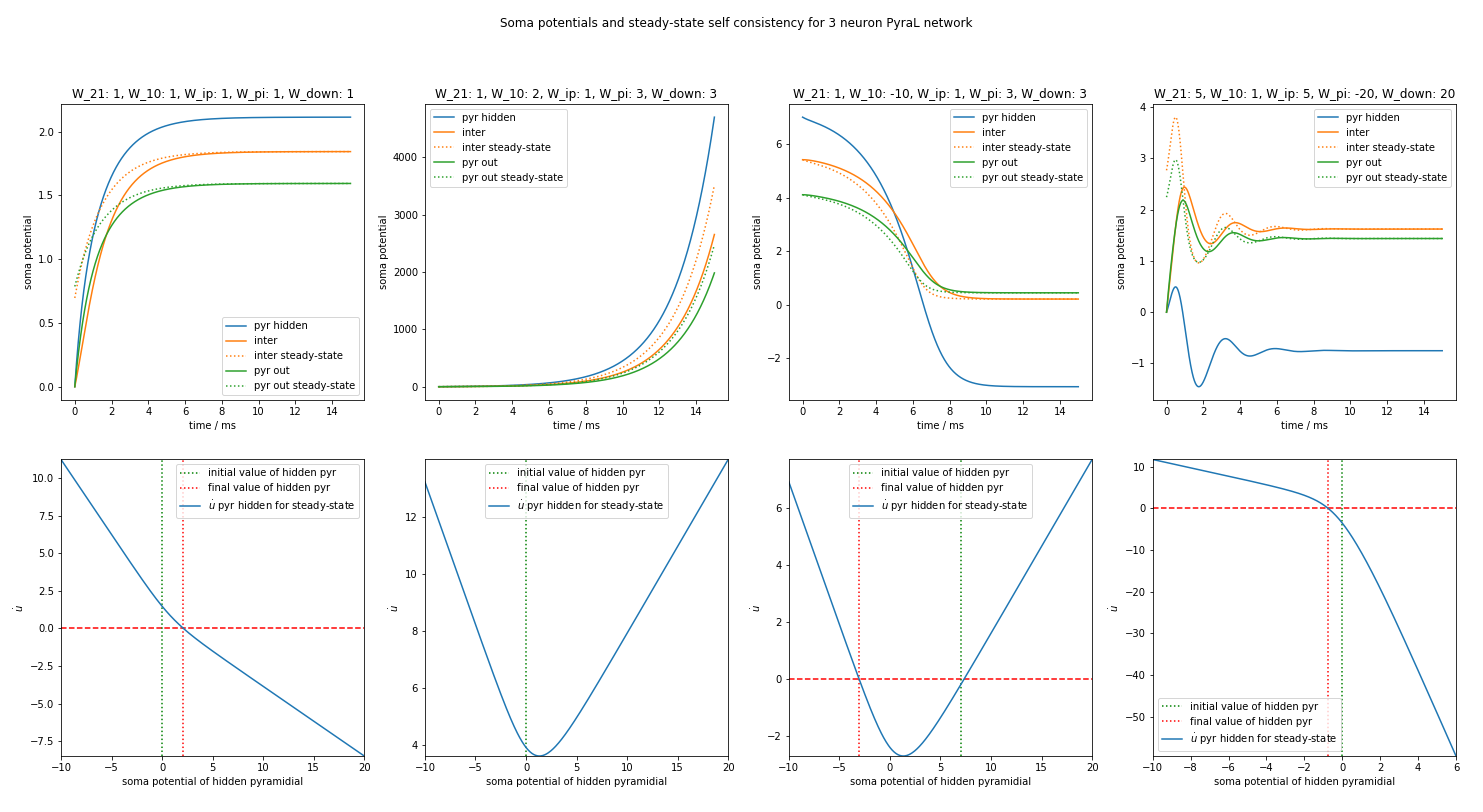
\includegraphics[width=\linewidth]{img/stability.png}
  \label{fig:stability}
  \caption{\textbf{Upper row}: Evolution of soma potentials of a simple 3-layer network with three neurons in total. Columns represent different network configurations and initial conditions and weights are kept fixed during the simulation. \textbf{Lower row}: Derivative of the hidden pyramidial soma potential $u^P_{hid}$ fully expressed through $u^P_{hid}$ via the steady-state solution of the other soma potential (see main text). \textbf{Details: } $g_A = g_{som} = 0.8$, $g_D = g_B = 1$, $g_l = 0.1$, $r_{in} = u^{target} = 1$, $dt = 0.001$}
\end{figure*}

Let us first investigate the network dynamics eq. \eqref{eq:dyn_hidden} - \eqref{eq:dyn_out}, i.e. with fixed weights, regarding stability. To do so we set up a very simple toy model with one hidden and output layer, each consisting of one pyramidial and one interneuron, one pyramidial output-neuron, respectively. A soft ReLU activation function ($\phi(u) = \ln(1 + \exp(u))$) is used since it is more prone to instabilities due to its unbound nature. Fig \ref{fig:stability} shows the behavior of the network for four different configurations of the network, where synaptic strengths and initial condition change. The input rate $r_{in}$ and the teaching potential $u_{target}$ is given and are equal for all cases. In the upper row the soma potentials of the three neurons are plotted, as well as the steady state solutions eq. \eqref{eq:steady} for the interneuron and the output-neuron given the current potential of the hidden pyramidial neuron.
In order for the system to posses a fix-point the left hand side of eq. \eqref{eq:dyn_hidden} - \eqref{eq:dyn_out} has to vanish simultaneously, i.e. at the fix-point
\begin{align}
u^{P}_{out} &= \frac{1}{g^{out}_{tot}}\left( g_B W_{21}\phi(u^P_{hid}) + g_{som}u^{target}\right) \label{eq:fix_out}\\
u^{I}_{hid} &= \frac{1}{g^{I}_{tot}}\left( g_D W_{ip}\phi(u^P_{hid}) + g_{som}u^{P}_{out}\right) \label{eq:fix_inter}\\
\dot{u}^P_{hid} &= -g^{P}_{tot}u^P_{hid} + g_B W_{10}r_{in} + g_A\left(W_{pi}\phi(u^I_{hid}) + W_{down}\phi(u^P_{out})\right) = 0 \label{eq:fix_pyr}
\end{align}
holds. Plugging \eqref{eq:fix_out}, \eqref{eq:fix_inter} into \eqref{eq:fix_pyr} yields the self-consistency condition
\begin{align*}
0 = \dot{u}^P_{hid} \equiv \dot{u}(u^P_{hid}) = ~&g^P_{tot}u^P_{hid} + g_B W_{10}r_{in} \\
&+ g_AW_{pi}\phi\left[\frac{1}{g^I_{tot}}\left( g_D W_{ip}\phi(u^P_{hid}) + \frac{g_{som}}{g^{out}_{tot}}\left( g_B W_{21}\phi(u^P_{hid}) + g_{som}u^{target}\right)\right)\right] \\
&+ g_AW_{down}\phi\left[\frac{1}{g^{out}_{tot}}\left( g_B W_{21}\phi(u^P_{hid}) + g_{som}u^{target}\right)\right]\\
\end{align*}
which is depicted in the lower row in Fig. \ref{fig:stability}. For the example configuration shown there, one finds a stable fix-point (first and last column), a stable and an unstable fix-point (third column) and no fix-point at all (second column). For the latter case the network behaves completely unstable and no mapping between in and output signals in the sense of the usual artificial neural networks exist. Also interesting is the last column in Fig. \ref{fig:stability} where an oscillatory behavior can be observed.


\subsubsection{Basic Regression Task and Emergence of Self-Predicting-State}
\begin{figure*}[!ht]
  \centering
  \subfigure[Output layer soma potentials and target potentials before training.]{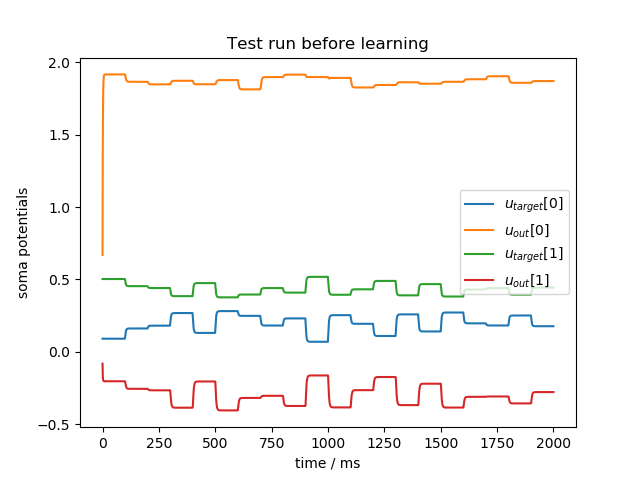
\includegraphics[height=0.35\linewidth]{img/PyraLNet/mimic_task/test_run_output_before.png}}\quad
  \subfigure[Output layer soma potentials and target potentials after training.]{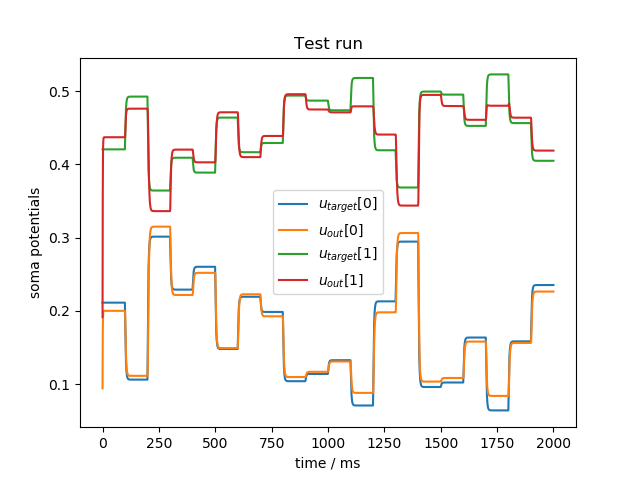
\includegraphics[height=0.35\linewidth]{img/PyraLNet/mimic_task/test_run_output.png}}\quad
  \subfigure[MSQE validation error during training.]{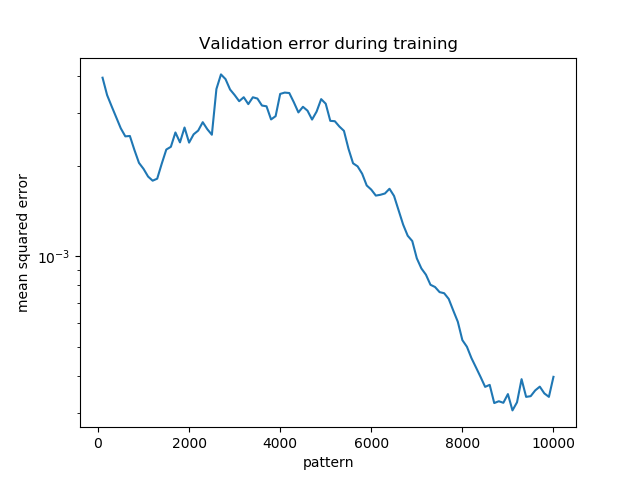
\includegraphics[height=0.35\linewidth]{img/PyraLNet/mimic_task/validation_error_during_training.png}}\quad
  \subfigure[Emergence of self-predicting-state during training starting from randomly initialized connections.]{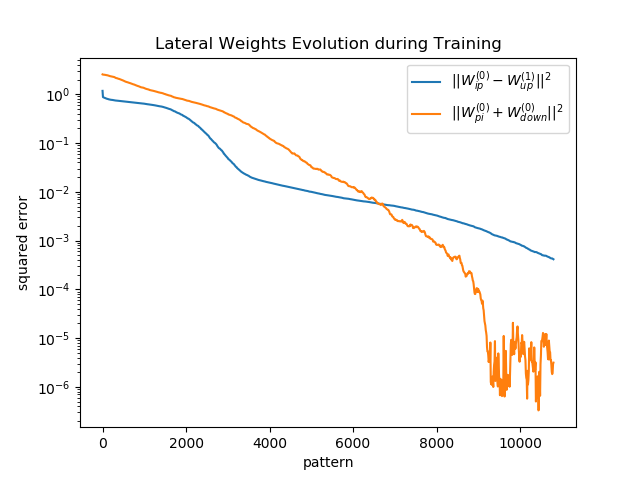
\includegraphics[height=0.35\linewidth]{img/PyraLNet/mimic_task/lateral_weights_during.png}}
  \label{fig:mimic}
\end{figure*}

As a first test setup we consider a simple "mimic-task" for a small network. We therefore devise a teaching network with only forwards weights as 
\begin{equation}
\bm{u}^{target} = \frac{g_B}{g_l + g_B} \bm{W}_{21}\phi\left(\frac{g_B}{g_l + g_B + g_A} \bm{W}_{10} \bm{r}_{in}\right),
\end{equation}
where the $g$s are the conductances of the network we want to train, such that both networks are garanteed to produce the same outputs once the self-predicting state has emerged and the forward weights of both networks equal (note that this must not necessarily be the case). The learning network is set up with the following parameters:
\begin{verbatim}
{"dims": [2, 3, 2], "dt": 0.1, "gl": 0.1, "gb": 1.0, "ga": 0.8, "gd": 1.0,
 "gsom": 0.8, "eta": {"up": [0.01, 0.005], "pi": [0.01, 0], "ip": [0.01, 0]},
 "bias": {"on": False, "val": 0.0},
 "init_weights": {"up": 1, "down": 1, "pi": 1, "ip": 1}, "tau_w": 30, "noise": 0,
 "t_pattern": 100, "out_lag": 3 * 10, "tau_0": 3, "learning_lag": 0,
 "reset_deltas": False}
\end{verbatim}

Let us go through this step by step. First the network dimensions are specified as input layer, hidden layer, ..., output layer dimension. Then we have the simulation parameter $dt$ used in the explicit Euler method for solving the network dynamics, followed by the conductances and the learning rates $\eta$ (\textit{eta}; order: first hidden layer to output layer). Next, one can specify whether a bias neuron, with fixed value \textit{val}, for the input and hidden layers should be added.\\
When the network is initialized all weights are drawn from a uniform distribution $U(-a,a)$, where $a$ can be specified per weight type in the next element. \textit{tau\_w} and \textit{t\_pattern} account for the plasticity time constant $\tau_w$ and the duration for which each input-output pair ($\bm{r}_{in},\bm{u}^{target}$) is presented, respectively. Furthermore these input-output signals are transitioned smoothly across patterns by applying a low-pass filter with time constant $\tau_0$ (\textit{tau\_0}). The noise parameter specifies the amount of Gaussian noise to add to the soma potential dynamics (this term is neglected in all of the above equations, see the original paper).\\
Interesting, however, are the remaining three parameters. \textit{out\_lag} specifies the amount of time to wait after each new input pattern, before the output potentials are averaged over the remaining pattern-time to give a single (time-independent) output vector associated to the presented input $\bm{r}_{in}$. Furthermore, it was observed, that the settling phase of the network contributes significantly to the overall prediction error during one pattern. This basically chokes learning of the problem beyond a certain threshold of accuracy, MSE of the potential deviations, respectively. In order to overcome this a so called learning-lag (\textit{learning\_lag}) was introduced, which specifies the amount of time to wait after a new pattern before plasticity is enabled, by means of eq. \eqref{eq:delta_up} - \eqref{eq:W_pi} (these equations are not invoked during that time). Additionally one can choose to set all updates $\Delta$ to zero after each pattern (if \textit{learning\_lag} $> 0$) by specifying \textit{reset\_deltas} accordingly.\\

Fig. \ref{fig:mimic} presents a network with the above parameters and a soft ReLU activation function that learned to mimic a teacher-network on a training set of 1000 points for 10 epochs. The upper row shows the output and target potentials before and after learning. The lower panel shows the mean squared error on validation samples (during which teaching is disabled) on the left. On the right one can observe the emergence of the self-predicting state during training as defined by eq. \eqref{eq:sps_pi} and \eqref{eq:sps_ip}, which leads to a drop in validation error.


\subsubsection{Steady-State-Approximation}
\begin{figure*}[!ht]
  \centering
  \subfigure[Deviation\protect\footnotemark ~of the simulated from the approximation soma potentials, when plasticity is switched off.]{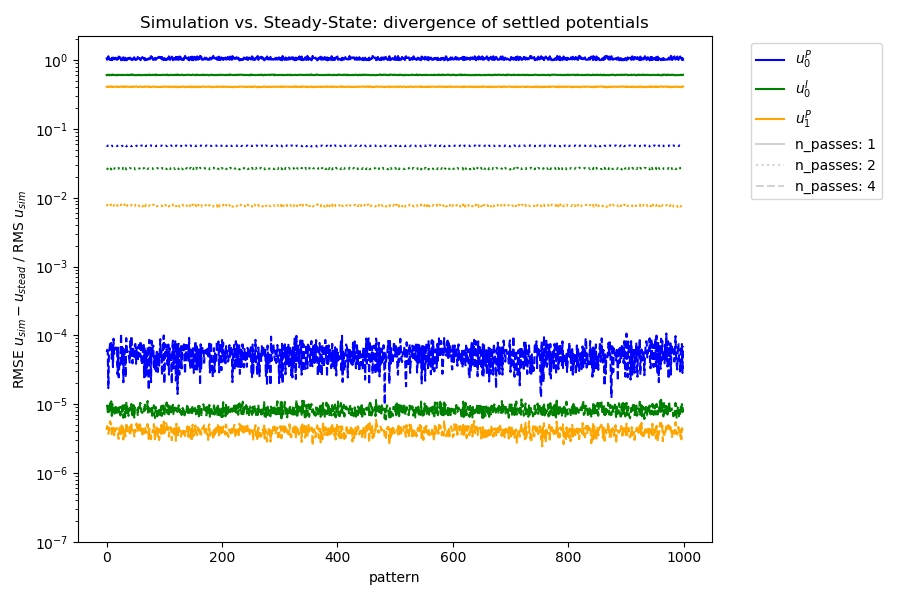
\includegraphics[height=0.32\linewidth]{img/SteadNet/stead_vs_sim/div_pots.png}}\quad
  \subfigure[Deviation of the simulated from the approximation soma potentials, when plasticity is switched off, but the network is initialized in the self-predicting state.]{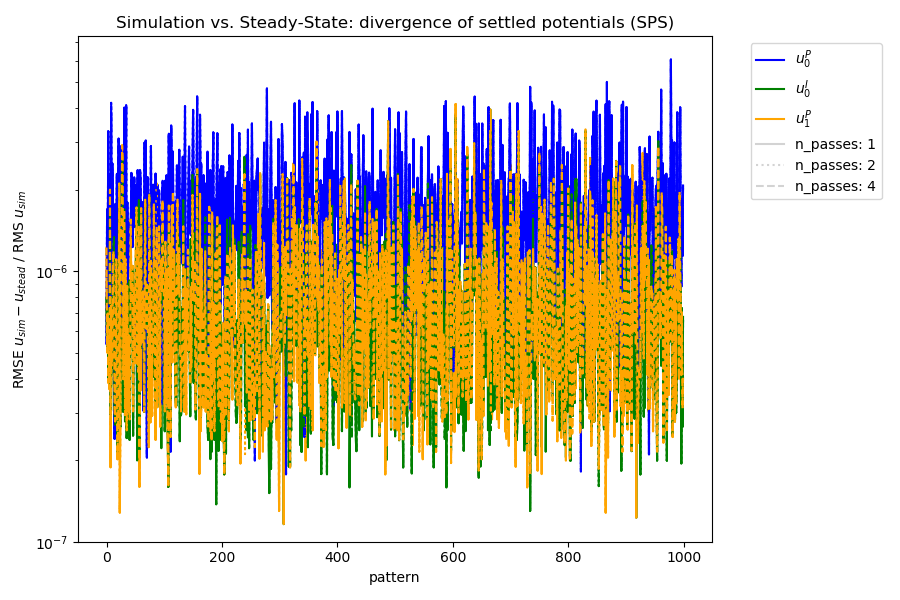
\includegraphics[height=0.32\linewidth]{img/SteadNet/stead_vs_sim/div_pots_sps.png}}\quad
  \subfigure[Deviation of the simulated from the approximation weights, when plasticity is switched on.]{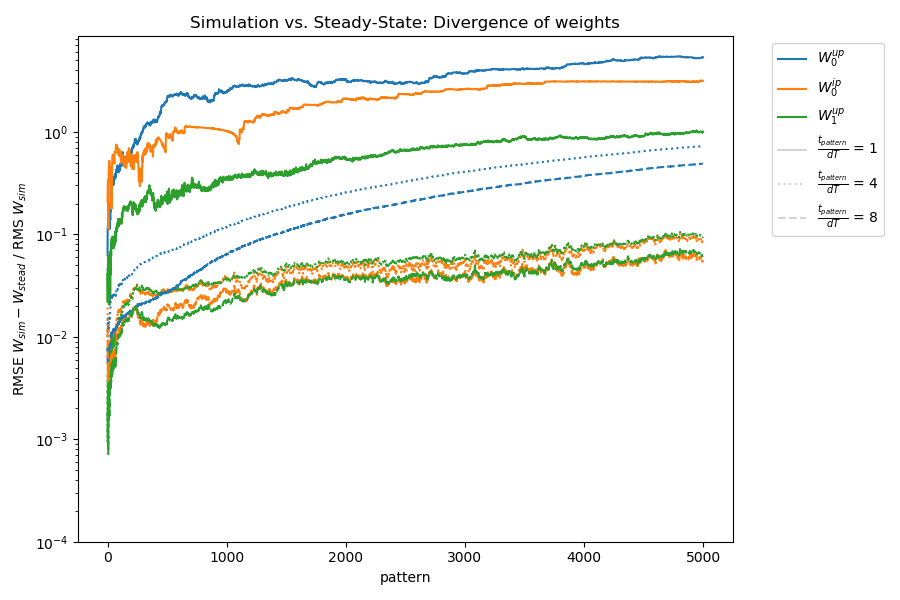
\includegraphics[height=0.32\linewidth]{img/SteadNet/stead_vs_sim/div_weights.png}}\quad
  \subfigure[Deviation of the simulated from the approximation weights, when plasticity is switched on, but the network is initialized in the self-predicting state.]{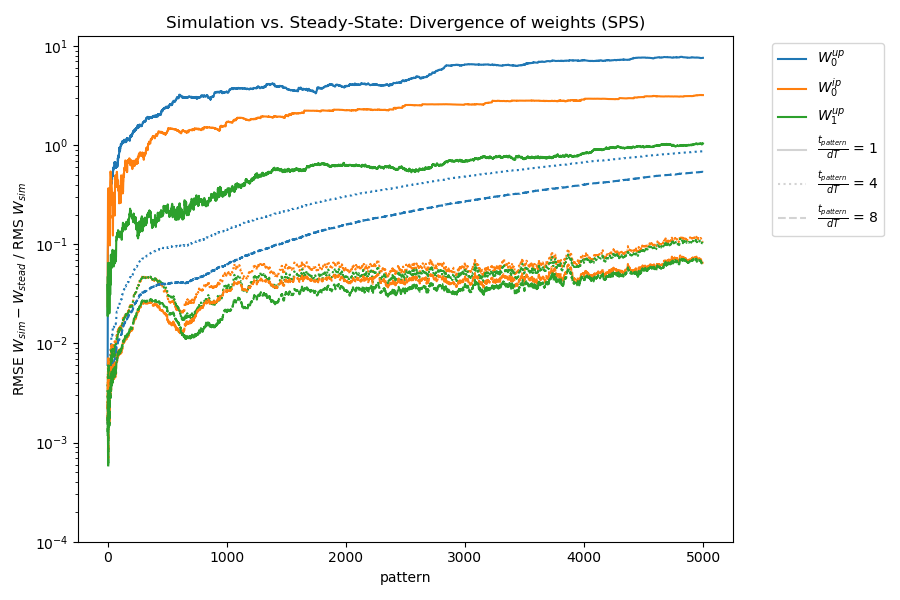
\includegraphics[height=0.32\linewidth]{img/SteadNet/stead_vs_sim/div_weights_sps.png}}
  \label{fig:stead}
\end{figure*}
\footnotetext{The deviation of the two vector or matrix quantities $\bm{a}$ and $\bm{b}$ w.r.t. $\bm{a}$ is defined as $\text{dev}(n) = \sqrt{\sum_i\left[(a_i(n)-b_i(n))^2 / \sum_na_i(n)^2\right]}$, where $i$ runs over the indices and $n$ is the pattern index. For the simulation-quantities (with time-dependence within one pattern) $n$ is associated with the last value per pattern.}

We now turn to evaluate the validity of the steady-state approximation approach. To this end we run a 4x120x3 sigmoid-network on the YinYang-training data (with nudging enabled) with the following parameters:
\begin{verbatim}
{"dims": [4, 120, 3], "dt": 0.1, "gl": 0.1, "gb": 1.0, "ga": 0.8, "gd": 1.0,
 "gsom": 0.8, "eta": {"up": [0.1, 0.01], "pi": [0.01, 0], "ip": [0.02, 0]},
 "bias": {"on": False, "val": 0.5},
 "init_weights": {"up": 0.5, "down": 0.5, "pi": 0.5, "ip": 0.5}, "tau_w": 30,
 "noise": 0, "t_pattern": 100, "out_lag": 80, "tau_0": 3, "learning_lag": 0,
 "reset_deltas": False}
\end{verbatim}
The upper left panel in Fig. \ref{fig:stead} shows the mean deviation of the soma potentials of the simulated and the steady-state network (for all three neuron types present) when plasticity is turned off (all $\eta$s are zero). The experiment is repeated for three different values of the SteadNet parameter \textit{n\_passes}, which gives the number the cycles in the steady-state approximation algorithm (cf. chapter \ref{chap:steadnet}). As one would expect, a higher value leads to a better approximation. Further note that no additional error builds up when multiple patterns are applied. In the upper right panel we see the same quantities but for a network initialized in the self-predicting state. Here the parameter \textit{n\_passes} doesn't lead to a significant decrease of the error. This can be anticipated since in the self-predicting state feeback contributions, except for the contribution of the target signal, mostly cancel.\\
For the lower panels plasticity was switched on. One can observe how the SteadNet parameter \textit{n\_exposures} leads to decreasing deviation between the weights of the simulation and the steady-state approximation. There is, however, little difference between the initial state of the network. In contrast to the soma potentials, the weight-error increasing with the number of patterns presented to the network.\\
Finally, note that the presented behavior strongly depends on the network parameters and might be significantly worse for larger weights or feedback conductances. Also a ReLU-like activation function would lead to worse deviations in most cases.


\subsection{MNIST with SteadNet}


\subsection{YinYang-Task}
For the YinYang-task it was found that the plasticity induced during the settling phase of the network restricted the performance of the network significantly. With a learning-lag of $20\text{ms}$ the best set of parameters found was 
\begin{verbatim}
{"dims": [4, 120, 3], "dt": 0.1, "gl": 0.1, "gb": 1.0, "ga": 0.28, "gd": 1.0,
 "gsom": 0.34, "eta": {"up": [6.1, 0.00012], "pi": [0, 0], "ip": [0.00024, 0]},
 "bias": {"on": True, "val": 0.5},
 "init_weights": {"up": 0.1, "down": 1, "pi": 1, "ip": 0.1}, "tau_w": 30, "noise": 0,
 "t_pattern": 100, "out_lag": 80, "tau_0": 3, "learning_lag": 20,
 "reset_deltas": False},
\end{verbatim}
where the parameters $g_{som}, g_A$ and $\eta^{up}_{1,2}$ where optimized ($\eta^{ip} = 2\eta^{up}_2$). For simplicity the network was initialized in the self-predicting state and lateral plasticity of the inter- to pyramidial neurons was switched off. The network was then trained on the YinYang-dataset (with normal and inverted coordinate inputs), where the labels where one-hot coded to the three output neurons of the network (logical zero was mapped to $0.1$ and logical one to $1.0$). A training set of 6000 samples was used and the network was trained for 45 epochs. After each epoch the progress was validated on a separate validation set (choose 100 samples at random from the validation set of size 600). With statistics taken from 10 runs with different seeds the network achieved an accuracy of
\begin{align*}
(96.7 \pm 0.76)\% \protect\footnotemark.
\end{align*}
\footnotetext{more precisely this is the result for \textit{learning\_lag} = 20.34 ms}

To further investigate the impact of the learning-lag the runs were repeated for different learning-lags and pattern durations $t_{pattern}$ (therefore also \textit{out\_lag} was adapted). 
The upper panels in Fig. \ref{fig:yinyang_vary} show the results for \textit{reset\_deltas} turned on and off, respectively. Mostly importantly this results indicate that simply increasing $t_{pattern}$ does not suffice to remove the unwanted plasticity induced during settling. One might argue that a simultaneous decrease of the learning-rates would lead to a significant improvement, however this comes at the cost of training-time. Further note that increasing learning-lag leads to a, so far unexpected, dip in performance around 5 ms. For low $t_{pattern}$ this effect is overcome be resetting the $\Delta$s after each pattern as can be observed in the left upper panel.\\
Furthermore, the impact of the effect of the parameters $\tau_0$ and $\tau_w$ was investigated. The results are presented in Fig. \ref{fig:yinyang_vary} in the lower panels. However, no interesting effect was found.


\begin{figure*}[!ht]
  \centering
  \subfigure[Output layer soma potentials and target potentials before training.]{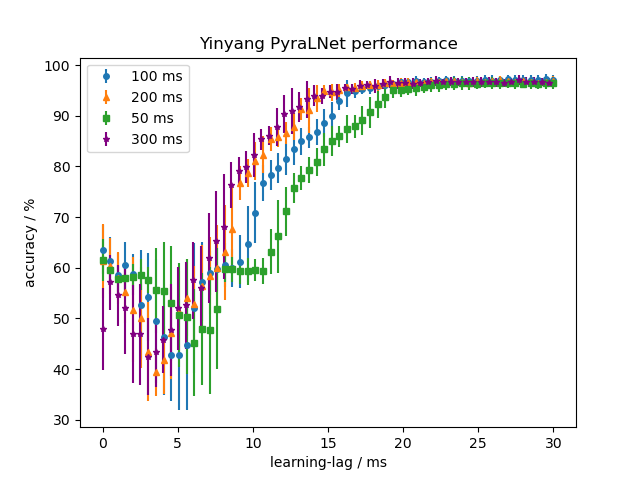
\includegraphics[height=0.35\linewidth]{img/eval/yinyang_acc_vs_llag.png}}\quad
  \subfigure[Output layer soma potentials and target potentials after training.]{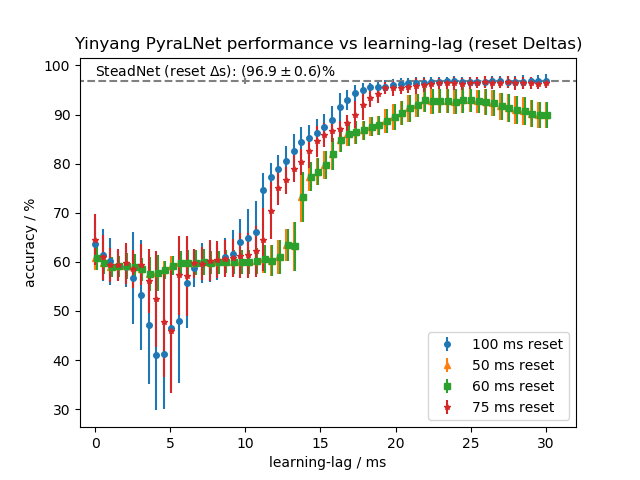
\includegraphics[height=0.35\linewidth]{img/eval/yinyang_acc_vs_llag_res_dels.png}}\quad
  \subfigure[MSQE validation error during training.]{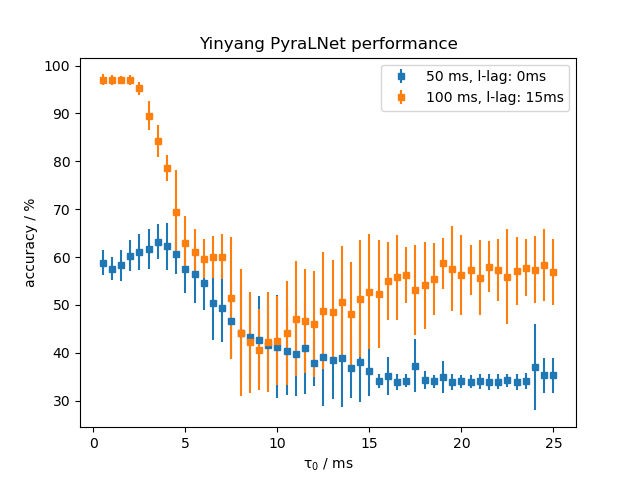
\includegraphics[height=0.35\linewidth]{img/eval/yinyang_acc_vs_tau_0.png}}\quad
  \subfigure[Emergence of self-predicting-state during training starting from randomly initialized connections.]{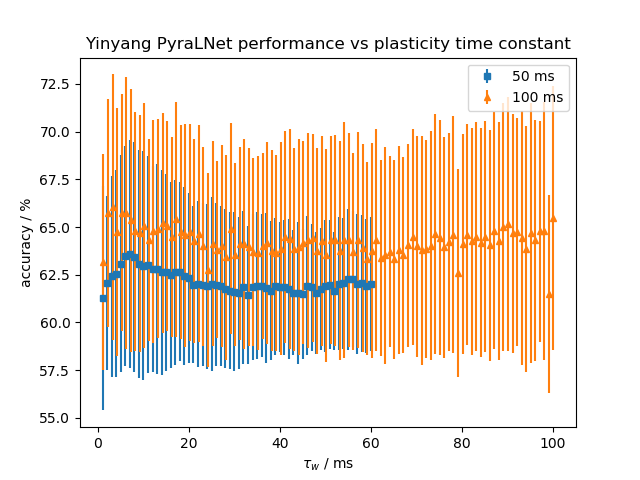
\includegraphics[height=0.35\linewidth]{img/eval/yinyang_acc_vs_tau_w.png}}
  \label{fig:yinyang_vary}
\end{figure*}

Finally, Fig. \ref{fig:yinyang_sps} shows how learning is still possible if the network is not initialized in the self-predicting state. To obtain this results the parameter $\eta_{pi}$ was optimized. The best results were found for $\eta_{pi}$

\begin{figure*}[!ht]
  \centering
  \subfigure[Output layer soma potentials and target potentials before training.]{\includegraphics[width=\linewidth]{img/best_sps_result.png}}\quad
  \subfigure[Output layer soma potentials and target potentials after training.]{\includegraphics[width=0.5\linewidth]{img/best_sps_weights.png}}
  \label{fig:yinyang_sps}
\end{figure*}

\end{document}
